\section{Ethylene carbonate with Na/Li TFSI salt}
\label{section:carbonates-structural}

Ethylene carbonate (EC) is one of the most widely used solvents for ion-conducting electrolytes due to its stability~\cite{lib-review}. To reduce the flammability, the addition of fluorinated derivatives of EC was considered and tested in lithium and sodium batteries~\cite{fluorination-1,fluorination-2,fluorination-3,fluorination-4}. This section presents results obtained for electrolytes based on LiTFSI or NaTFSI dissolved in EC or in its mono- (F1EC) and diflorinated (F2EC) derivatives, as well as for neat solvent, which were a~subject of experimental work~\cite{fluorination-2}. This study was published in the~paper~\cite{carbonates}.

\subsection{System details}

QC calculations were performed in vacuum using MP2 methodology to determine the Na$^{+}$-carbonate binding energies and to obtain the IR spectra. 

\begin{table}[ht]
    \centering
    \caption{Compositions of Li/NaTFSI - carbonate systems}
    \label{tab:carbonates-compositions}
\begin{tabular}{ccccc}
\toprule
system     & carbonate & MeTFSI & atoms & concentration, mol/dm3 \\
\midrule
EC         & 500       & 0      & 5000  & 0                      \\
F1EC       & 500       & 0      & 5000  & 0                      \\
F2EC       & 500       & 0      & 5000  & 0                      \\
Li-EC      & 474       & 41     & 5396  & 1.072                  \\
Li-EC      & 348       & 127    & 5512  & 2.922                  \\
Li-F1EC    & 466       & 42     & 5332  & 1.034                  \\
Li-F2EC    & 461       & 47     & 5362  & 1.065                  \\
Li-EC/F1EC & 235/235   & 41     & 5356  & 1.041                  \\
Na-EC      & 474       & 41     & 5396  & 1.065                  \\
Na-EC      & 348       & 127    & 5512  & 2.875                  \\
Na-F1EC    & 466       & 42     & 5332  & 1.028                  \\
Na-F2EC    & 461       & 47     & 5362  & 1.055                  \\
Na-EC/F1EC & 235/235   & 41     & 5356  & 1.034                  \\
\bottomrule
\end{tabular}
\end{table}

The compositions of the systems simulated in classical MD are listed in Table~\ref{tab:carbonates-compositions}. Simulations were performed under the 1~atm pressure, and in temperature of 298~K for 20~ns, and then 150~ns of trajectories were produced in the NVT ensemble, the last 100~ns was used for analysis. The time step was equal 1.0~fs.

AIMD simulations were performed for selected systems: neat solvents, Li/NaTFSI in EC and for LiTFSI in F1EC. Simulation boxes contained 50~solvent molecules (for neat solvents) or 46 solvent molecules and 4 MeTFSI ion pairs. Simulations were performed with 1.0~fs timestep for 35~ps, for analysis the last 30~ps were used.

\subsection{Results}

The binding energies calculated at the MP2 level are listed in Table~\ref{tab:carbonates-binding-energies}. It is readily seen that the binding of Na$^{+}$ is weaker than that of Li$^{+}$ and that for both ions, the strength of the binding decreases in the order EC > F1EC > F2EC.

\begin{table}[ht]
  \centering
  \caption[Binding energies in kcal/mol calculated at the MP2 level]{Binding energies in kcal/mol calculated at the MP2 level, data for Li$^{+}$ are taken from~\cite{carbonates-li-binding-energies}}
  \label{tab:carbonates-binding-energies}
\begin{tabular}{cccc}
\toprule
cation/carbonate & EC    & F1EC  & F2EC  \\
\midrule
Li$^{+}$               & -46.9 & -42.2 & -37.1 \\
Na$^{+}$               & -38.2 & -34.3 & -30.2 \\
\bottomrule
\end{tabular}
\end{table}

The RDFs for the Me-O$_{\text{carb}}$ pairs are presented in Figure~\ref{fig:carbonates-figure-1}. The positions of the first maximum do not depend on the carbonate used as a~solvent and are equal 1.91~{\AA} for lithium and 2.31-2.32~{\AA} for sodium in 1~M solutions. The value for lithium agrees with experimentally measured 1.91~{\AA} by neutron diffraction~\cite{neutron-diffraction}. In AIMD, both maxima appear at higher distances, 1.95 and 1.97~{\AA} for lithium in EC and F1EC respectively and at 2.38~{\AA} for sodium in EC.

\begin{figure}[ht]
    \centering
    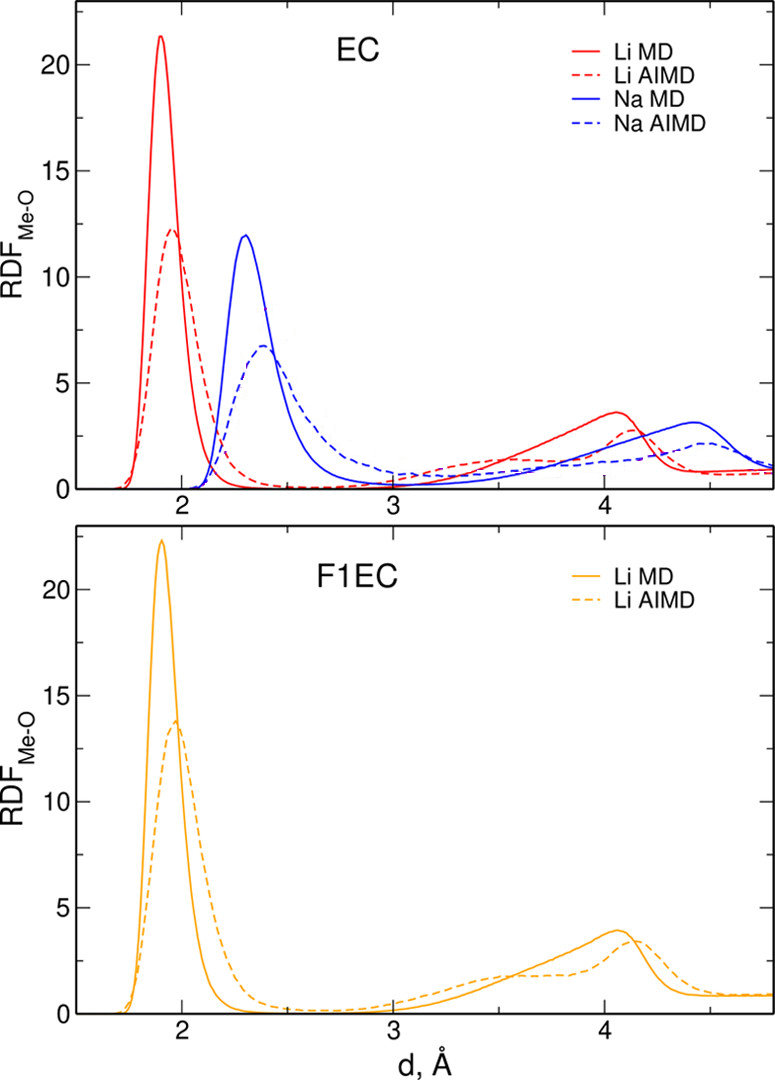
\includegraphics[width=0.4\textwidth]{img/3-structural-data-from-md-simulations/4-carbonates/figure1.png}
    \caption{Radial distribution functions for Me-O$_{\text{carb}}$ pairs where O$_{\text{carb}}$ is the oxygen atom from carbonate molecule}
    \label{fig:carbonates-figure-1}
\end{figure}

\begin{figure}[ht]
    \centering
    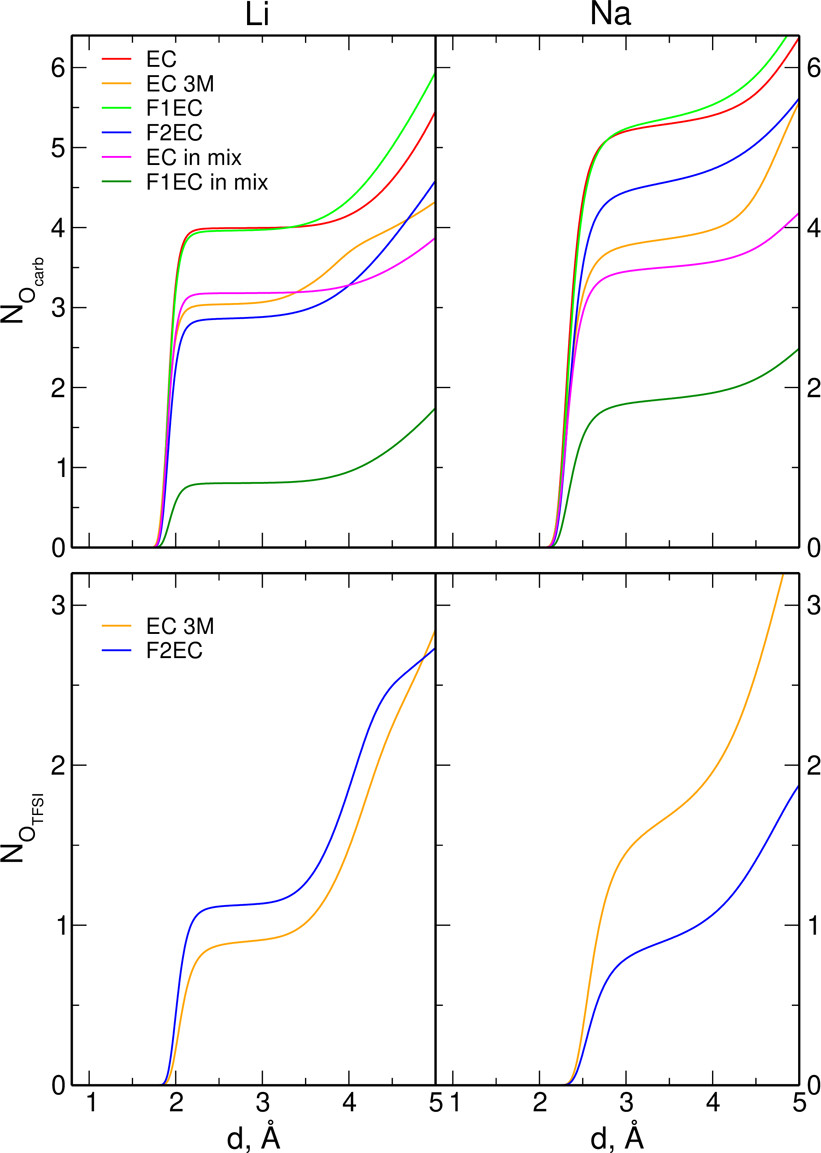
\includegraphics[width=0.4\textwidth]{img/3-structural-data-from-md-simulations/4-carbonates/figure2.png}
    \caption{Integrated Me-O RDFs from classical MD for carbonate and TFSI oxygen atoms}
    \label{fig:carbonates-figure-2}
\end{figure}

In Figure~\ref{fig:carbonates-figure-2} integrated RDFs for Me-O pairs are shown. Non-negligible coordination by the TFSI$^{-}$ anion is observed only in the case of F2EC or concentrated (3~M) solutions, thus only these results are presented. For lithium cations, coordination numbers in 1~M solutions are similar for EC and F1EC and equal~4. Similarly, for sodium these numbers are equal 5.3 and 5.37 respectively and are larger due to the bigger cation radius. For F2EC solutions, the number of coordinating oxygens from carbonate molecules decreases to 2.88 and 4.58 for lithium and sodium, respectively. However, in this case the average number of coordinating oxygen atoms from the TFSI$^{-}$ anion are equal 1.14 and 0.91 respectively, leading to total coordination numbers equal 4.02 and 5.49 respectively. Similarly, these total values remain unaffected for 1:1 EC/F1EC solvent mixture. However, in this case, ratios of coordinating EC and F1EC are not 1:1, but are 3.18:0.81 for lithium and 3.51:1.86 for sodium, respectively. This shows that coordination to EC is preferred over F1EC and is in agreement with results of electrospray ionization mass spectroscopy experiments~\cite{vibrational-exp-3}. In 3~M solutions in EC the average number of coordinating oxygen atoms are equal 3.07 O$_{\text{carb}}$ and 0.91 O$_{\text{TFSI}}$ for lithium and 3.86 O$_{\text{carb}}$ and 1.69 O$_{\text{TFSI}}$ for sodium, respectively. Thus, here high concentration increased the probability of coordination by TFSI$^{-}$ anions. In case of F2EC solutions non-negligible coordination by TFSI$^{-}$ anion is caused by Me-solvent binding weaker than in EC or F1EC solutions.

\begin{figure}[H]
    \centering
    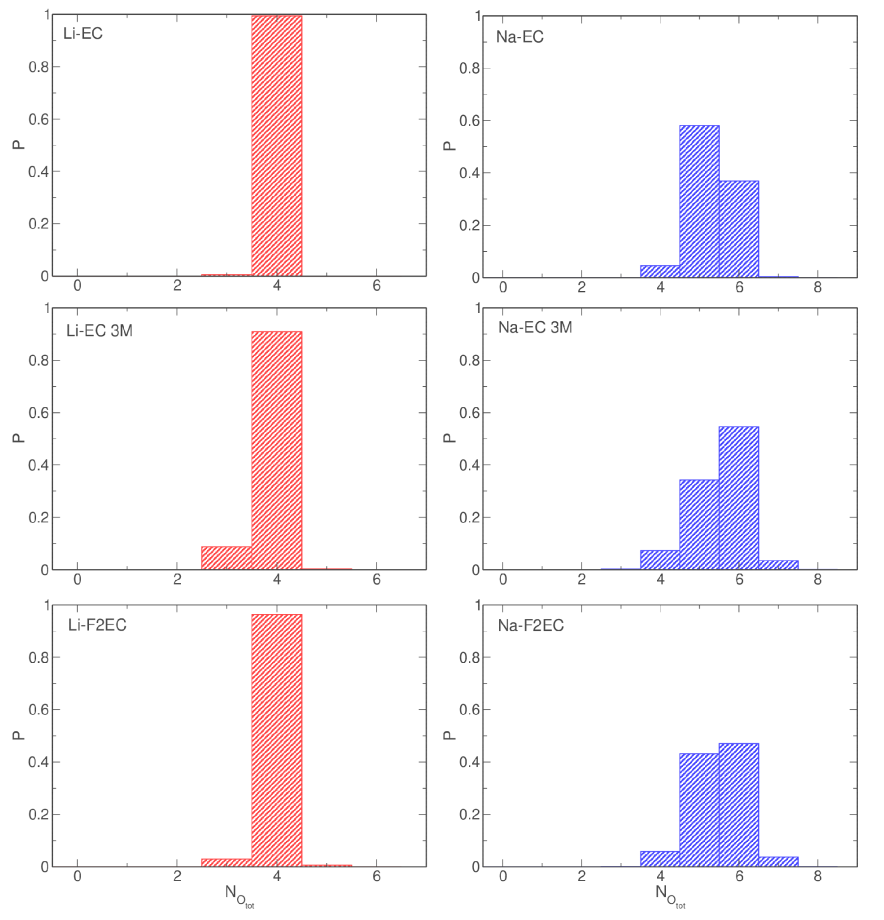
\includegraphics[width=0.5\textwidth]{img/3-structural-data-from-md-simulations/4-carbonates/histogram-o-atoms.png}
    \caption{Histograms of average total numbers of oxygen atoms coordinating the Me$^{+}$ ion}
    \label{fig:carbonates-histogram-o-atoms}
\end{figure}

Figure~\ref{fig:carbonates-histogram-o-atoms} contains example histograms of total number of coordinating oxygen atoms for metal cations. For lithium, in almost all cases, the most probable number of oxygen atoms is~4, only in the 3~M solution there is about 10\% of ions with coordination number equal~3. For sodium cation most probable is coordination by either 5~or 6~oxygen atoms, higher values are preferred in fluorinated solvents or in the concentrated solution. From the histograms (not shown here, but presented in~\cite{carbonates}) for specific oxygen atoms (from solvent or TFSI$^{-}$ anion) it is observed that in most cases the cation is coordinated only by solvent molecules and the total coordination number is equal to the number of coordinating solvent molecules. The only exceptions are solutions in F2EC or 3~M in EC. In these systems, the possible O$_{\text{TFSI}}$ values range from 0~to 4~for Li$^{+}$ and from 0~to 6~for Na$^{+}$, however 0~is the most probable number (40-55\%). Even values of O$_{\text{TFSI}}$ number seem to be favored and together with the observation that the number of coordinating TFSI$^{-}$ anions is usually between 0~and~2, this leads to conclusion that bidentate Me$^{+}$ coordination by the anions is preferred.

\begin{table}[ht]
  \centering
  \caption{Residence times in ns for oxygen atoms from solvent molecules or TFSI$^{-}$ anions and anion residence times}
  \label{tab:carbonates-residence}
\begin{tabular}{cccccc}
\toprule
           &      &      &      & \multicolumn{2}{c}{TFSI} \\
system     & EC   & F1EC & F2EC & $\tau_O$         & $\tau_{\text{an}}$         \\
\midrule
Li-EC      & 7.6  &      &      &            &             \\
Li-EC 3 M  & 37.4 &      &      & 3.8        & 13.6        \\
Li-F1EC    &      & 3.6  &      &            &             \\
Li-F2EC    &      &      & 1.9  & 3.7        & 12.4        \\
Li-EC/F1EC & 12.0 & 2.3  &      &            &             \\
Na-EC      & 1.5  &      &      &            &             \\
Na-EC 3 M  & 19.1 &      &      & 2.9        & 10.9        \\
Na-F1EC    &      & 1.4  &      &            &             \\
Na-F2EC    &      &      & 1.0  & 0.7        & 2.4         \\
Na-EC/F1EC & 2.5  & 0.9  &      &            &             \\
\bottomrule
\end{tabular}
\end{table}

To study the dynamics of complexation, residence time autocorrelation functions were calculated. Their plots are presented in Figures~\ref{fig:carbonates-figure-3} and~\ref{fig:carbonates-figure-4}. For each of them stretched exponential functions $e^{-\left( \frac{t}{\tau_O} \right)^{\alpha}}$ were fitted yielding the residence times $\tau_O$ which are collected in Table~\ref{tab:carbonates-residence}. For every case, values for lithium are larger than for sodium and regardless of the cation they decrease in order EC > F1EC > F2EC. This implies faster exchange of solvent molecules in solvation shell for fluorinated ones what agrees with tendencies observed for binding energies from QC calculations. In concentrated electrolytes, solvent residence times increase by about an order of magnitude, which is probably caused by the bigger viscosity of such systems. In EC:F1EC mixture residence times for EC molecules are larger than those in pure EC electrolyte and the opposite effect is observed for F1EC, thus in the solvent mixture, the stronger interacting solvent remains bound to the cation for longer times and the speed of exchange of the other solvent increases. For residence times for TFSI$^{-}$ anions and its oxygen atoms, in 3~M EC solutions values for sodium decrease about 20-30\% with respect to values for lithium, in this case the dynamics is presumably limited by the viscosity. In the case of 1~M solutions in F2EC, the decrease for sodium is about 5-fold when compared to lithium. 

\begin{figure}[H]
    \centering
    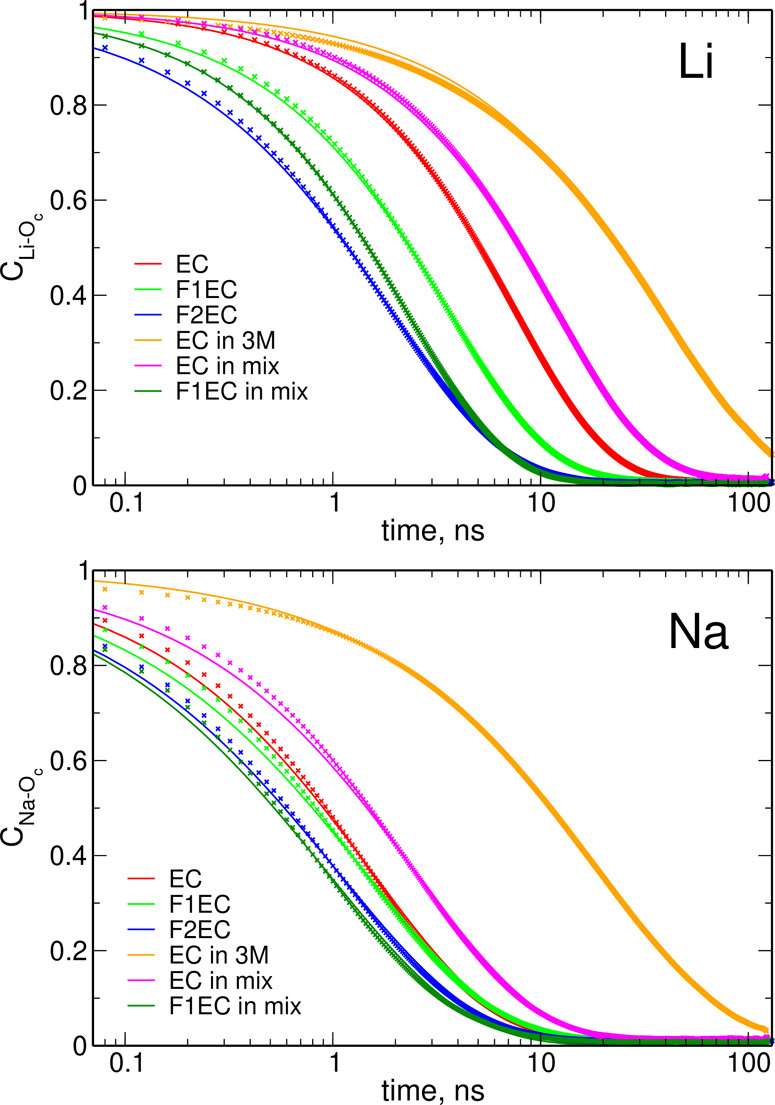
\includegraphics[width=0.4\textwidth]{img/3-structural-data-from-md-simulations/4-carbonates/figure3.png}
    \singlespacing
    \caption{Residence time autocorrelation functions for Me-O$_{\text{carb}}$, lines are fits to the data}
    \label{fig:carbonates-figure-3}
\end{figure}

\begin{figure}[H]
    \centering
    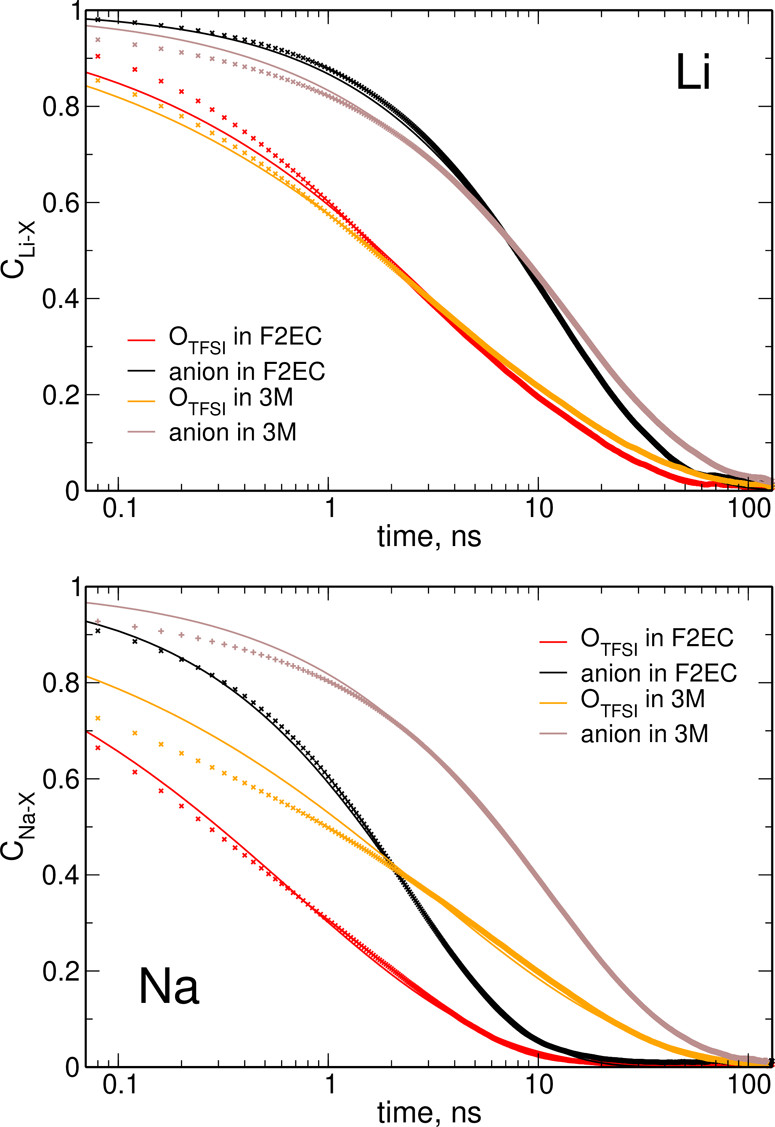
\includegraphics[width=0.4\textwidth]{img/3-structural-data-from-md-simulations/4-carbonates/figure4.png}
    \singlespacing
    \caption{Residence time autocorrelation functions for Me-O$_{\text{TFSI}}$ and Me-anion, lines are fits to the data}
    \label{fig:carbonates-figure-4}
\end{figure}

Observed differences between sodium and lithium-based electrolytes in the structure and dynamics are the effect of different strengths of cation-solvent interactions. Solutions in pure EC or F1EC do not differ significantly; however in electrolytes based on EC/F1EC mixture, cations prefer interactions with EC molecules. This trend may have an influence on the local structure and ion exchange in electrolytes with an F1EC additive, and it should be further investigated.

\cleardoublepage